\documentclass[unicode,11pt,a4paper,oneside,numbers=endperiod,openany]{scrartcl}

\usepackage{amsmath} 
\usepackage{amsfonts}
\usepackage{graphicx}
\usepackage{enumitem} 
\usepackage{longtable}
\usepackage{array}
\usepackage{xcolor}
\usepackage{booktabs}
\usepackage{multirow}
\usepackage{geometry}
\usepackage{listings}
\usepackage{subcaption}
\usepackage{caption} 
\lstdefinestyle{mystyle}{
    basicstyle=\ttfamily\small,
    keywordstyle=\color{blue},
    commentstyle=\color{green},
    stringstyle=\color{red},
    numbers=left,
    numberstyle=\tiny,
    stepnumber=1,
    frame=single,
    breaklines=true,
    captionpos=b,
    tabsize=2
}

\lstdefinelanguage{MyC++}{
    language=C++,
    morekeywords={std, vector, string},
}

\lstdefinelanguage{MyPython}{
    language=Python,
    morekeywords={self},
}

\lstdefinelanguage{MyBatch}{
    morekeywords={echo, pause, set},
    sensitive=false, 
    morecomment=[l]{REM}, 
    morestring=[b]",
}

\lstdefinelanguage{MyPython}{
    language=Python,
    morekeywords={self, int, float, str, list, dict, set, tuple, bool, None, True, False},
    keywordstyle=\color{blue},
    stringstyle=\color{red},
    commentstyle=\color{green},
    sensitive=true
}

\lstdefinelanguage{MyBash}{
    basicstyle=\ttfamily,
    breaklines=true,
    frame=single,
    keywordstyle=\color{blue},
    commentstyle=\color{gray},
    showstringspaces=false
}
\lstdefinelanguage{MyMATLAB}{
    language=Matlab,
    keywordstyle=\color{blue},
    stringstyle=\color{red},
    commentstyle=\color{green},
    morekeywords={struct, fullfile, csvread, issymmetric, sparse, accumarray, max, ones}
}
\usepackage{ifthen}
\usepackage[utf8]{inputenc}
\usepackage{graphics}
\usepackage{graphicx}
\usepackage{hyperref}

\pagestyle{plain}
\voffset -5mm
\oddsidemargin  0mm
\evensidemargin -11mm
\marginparwidth 2cm
\marginparsep 0pt
\topmargin 0mm
\headheight 0pt
\headsep 0pt
\topskip 0pt        
\textheight 255mm
\textwidth 165mm

\newcommand{\duedate} {}
\newcommand{\setduedate}[1]{%
\renewcommand\duedate {See iCorsi for due date}}
\newcommand\isassignment {false}
\newcommand{\setassignment}{\renewcommand\isassignment {true}}
\newcommand{\ifassignment}[1]{\ifthenelse{\boolean{\isassignment}}{#1}{}}
\newcommand{\ifnotassignment}[1]{\ifthenelse{\boolean{\isassignment}}{}{#1}}

\newcommand{\assignmentpolicy}{
\begin{table}[h]
\begin{center}
\scalebox{0.8} {%
\begin{tabular}{|p{0.02cm}p{16cm}|}
\hline
&\\
\multicolumn{2}{|c|}{\Large\textbf{HPC Lab ---  Submission Instructions}}\\
\multicolumn{2}{|c|}{\large\textbf{(Please, notice that following instructions are mandatory: }}\\
\multicolumn{2}{|c|}{\large\textbf{submissions that don't comply with, won't be considered)}}\\
&\\
\textbullet & Assignments must be submitted to \href{https://www.icorsi.ch}{iCorsi} (i.e. in electronic format).\\
\textbullet & Provide both executable package and sources (e.g. C/C++ files, Matlab). 
If you are using libraries, please add them in the file. Sources must be organized in directories called:\\
\multicolumn{2}{|c|}{\textit{Project\_number\_lastname\_firstname}}\\
& and  the  file must be called:\\
\multicolumn{2}{|c|}{\textit{project\_number\_lastname\_firstname.zip}}\\
\multicolumn{2}{|c|}{\textit{project\_number\_lastname\_firstname.pdf}}\\
\textbullet &  The TAs will grade your project by reviewing your project write-up, and looking at the implementation 
                 you attempted, and benchmarking your code's performance.\\

\textbullet & You are allowed to discuss all questions with anyone you like; however: (i) your submission must list anyone you discussed problems with and (ii) you must write up your submission independently.\\
\hline
\end{tabular}
}
\end{center}
\end{table}
}
\newcommand{\punkte}[1]{\hspace{1ex}\emph{\mdseries\hfill(#1~\ifcase#1{Points}\or{Points}\else{Points}\fi)}}


\newcommand\serieheader[6]{
\thispagestyle{empty}%
\begin{flushleft}

\includegraphics[width=0.4\textwidth]{usi_inf.png}
\end{flushleft}
  \noindent%
  {\large\ignorespaces{\textbf{#1}}\hspace{\fill}\ignorespaces{ \textbf{#2}}}\\ \\%
  {\large\ignorespaces #3 \hspace{\fill}\ignorespaces #4}\\
  \noindent%
  \bigskip
  \hrule\par\bigskip\noindent%
  \bigskip {\ignorespaces {\Large{\textbf{#5}}}
  \hspace{\fill}\ignorespaces \large \ifthenelse{\boolean{\isassignment}}{\duedate}{#6}}
  \hrule\par\bigskip\noindent%  \linebreak
 }

\makeatletter
\def\enumerateMod{\ifnum \@enumdepth >3 \@toodeep\else
      \advance\@enumdepth \@ne
      \edef\@enumctr{enum\romannumeral\the\@enumdepth}\list
      {\csname label\@enumctr\endcsname}{\usecounter
        {\@enumctr}%%%? the following differs from "enumerate"
	\topsep0pt%
	\partopsep0pt%
	\itemsep0pt%
	\def\makelabel##1{\hss\llap{##1}}}\fi}
\let\endenumerateMod =\endlist
\makeatother




\usepackage{textcomp}





\begin{document}


\setassignment

\serieheader{High-Performance Computing Lab}{Institute of Computing}{Student: ZITIAN WANG}{Discussed with: NULL}{Solution for Project 7}{}
\newline

\assignmentpolicy

% -------------------------------------------------------------------------- %
% -------------------------------------------------------------------------- %
% --- Exercise 1 ----------------------------------------------------------- %
% -------------------------------------------------------------------------- %
% -------------------------------------------------------------------------- %


\section{HPC Mathematical Software for Extreme-Scale Science  [85 points]}
The Poisson equation $-\Delta u = f$ on a unit square $\Omega = [0, 1] \times [0, 1]$ with Dirichlet boundary conditions $u = 0$ on $\partial \Omega$ is discretized on an $nx \times ny$ grid with spacings $dx = \frac{1}{nx-1}$ and $dy = \frac{1}{ny-1}$. The Laplacian $\Delta$ is approximated using the second-order centered finite difference formula $\Delta u \approx \frac{u_{i+1,j} + u_{i-1,j} - 2u_{i,j}}{dx^2} + \frac{u_{i,j+1} + u_{i,j-1} - 2u_{i,j}}{dy^2}$ for interior grid points. This discretization leads to a linear system $A\mathbf{u} = \mathbf{b}$, where $A$ is the matrix representation of the Laplacian, $\mathbf{u}$ is the vector of the unknowns at grid points, and $\mathbf{b}$ is the source term vector, uniformly filled with the constant $f$. Boundary conditions are applied by setting the corresponding elements of $\mathbf{u}$ to zero and adjusting $A$ accordingly.


\subsection{Boundary problem above in Python [25 points]}
\begin{lstlisting}[language=MyPython, style=mystyle, caption={Matrix and RHS Computation in Python}]
	def ComputeRHS(nx, ny, f_value):
		"""Compute the right-hand side vector."""
	
		# TODO Gernate RHS vector
		# Note .flatten() By default we have "row-major" ordering!
		rhs = np.full((nx * ny,), f_value)
		return rhs
	
	def ComputeMatrix(nx, ny, dx, dy):
	
		data = []
		row_indices = []
		col_indices = []
	
		N = nx * ny    
	
		# TODO: Loop over grid points (i, j) and compute the entries of matrix A as a sparse matrix by populating row_indices, col_indices, and data.
		for j in range(ny):
			for i in range(nx):
				index = j * nx + i
				if i == 0 or j == 0 or i == nx - 1 or j == ny - 1:
					row_indices.append(index)
					col_indices.append(index)
					data.append(1)
				else:
					row_indices.extend([index, index, index, index, index])
					col_indices.extend([index, index + 1, index - 1, index + nx, index - nx])
					data.extend([-4, 1, 1, 1, 1])
	
		return csr_matrix((data, (row_indices, col_indices)), shape=(N, N))
\end{lstlisting}
\begin{lstlisting}[language=MyBatch, style=mystyle, caption={Poisson Solver Output}]
	(petsc) [wangzi@icsnode26 poisson]$ python3 poisson_py.py 
	Selected solvers: ['sp_dir', 'dn_dir', 'sp_cg']
	------------------------------------------------------------------
	Poisson's Equation Solver Python for 64x18
	------------------------------------------------------------------
	RHS Time:                                0.000015 seconds
	Matrix Assembly Time:                    0.002577 seconds
	------------------------------------------------------------------
	Sparse Direct Solver Time:               0.002997 seconds, Norm of Solution: 14304.336841
	Dense Direct Solver Time:                0.047494 seconds, Norm of Solution: 14304.336841
	Conjugate Gradient (sparse) Solver Time: 0.585268 seconds, Norm of Solution: 14621.438228
	------------------------------------------------------------------
	Solution written to disk for solution_sp_dir ...
	Solution written to disk for solution_dn_dir ...
	Solution written to disk for solution_sp_cg ...
	\end{lstlisting}

% \begin{figure}[htbp]
%     \centering

%     % 第一行图片
%     \begin{subfigure}[b]{0.4\textwidth}
%         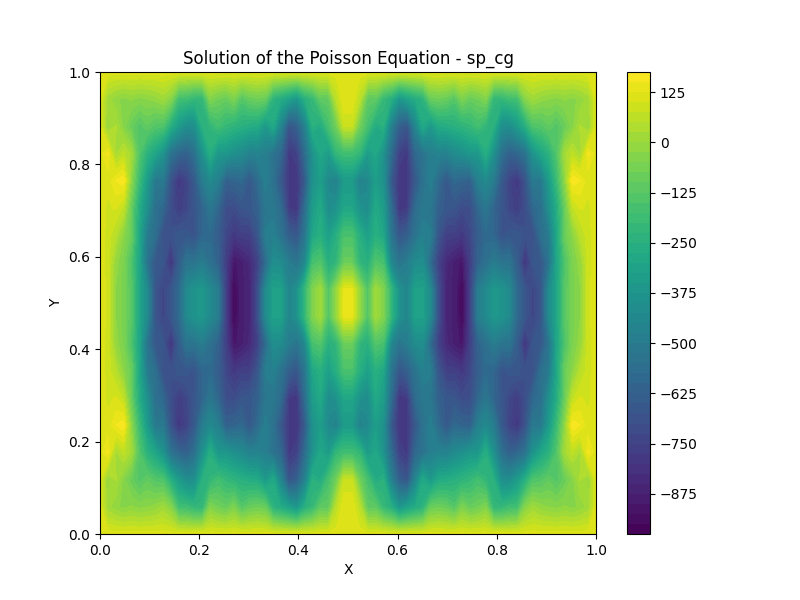
\includegraphics[width=\textwidth]{images/sp_cg_solution_plot.png}
%         \caption{sp\_cg\_solution}
%     \end{subfigure}
%     \hfill
%     \begin{subfigure}[b]{0.4\textwidth}
%         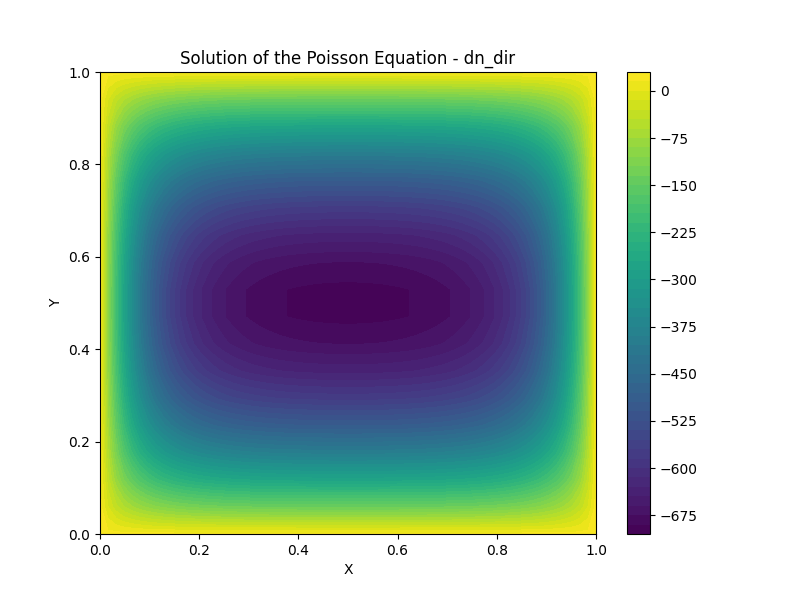
\includegraphics[width=\textwidth]{images/dn_dir_solution_plot.png}
%         \caption{dn\_dir\_solution}
%     \end{subfigure}

%     % 添加垂直空隙
%     \vspace{1em}

%     % 第二行图片
%     \begin{subfigure}[b]{0.4\textwidth}
%         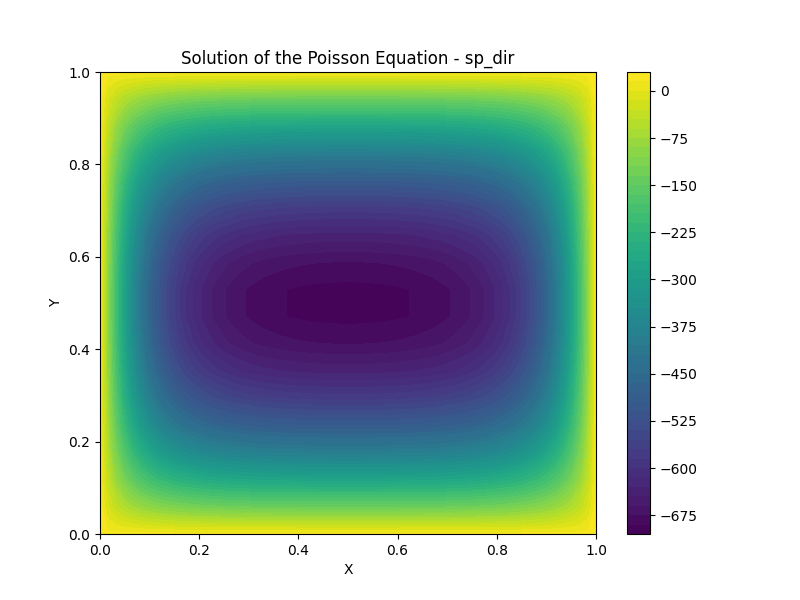
\includegraphics[width=\textwidth]{images/sp_dir_solution_plot.png}
%         \caption{sp\_dir\_solution}
%     \end{subfigure}

%     \caption{Comparison of solutions} % 整体标题
%     \label{fig:solution_comparison}
% \end{figure}

\subsection{Boundary problem above in PETSc [25 points]}
\begin{lstlisting}[language=MyC++, style=mystyle, caption={ComputeRHS function in PETSc C++ code}]
	PetscErrorCode ComputeRHS(KSP ksp, Vec b, void *ctx) {
	  UserContext   *user = (UserContext *)ctx;  // User-provided context for constant source term
	  DM             da;                         // Distributed array
	  DMDALocalInfo  info;                       // Local grid information
	  PetscScalar  **array;                      // Local portion of vector array
	  PetscReal      hx, hy;                     // Grid spacing in x and y directions
	  PetscInt       i, j;
	
	  PetscFunctionBeginUser;
	
	  // Get the distributed array and local grid information
	  PetscCall(KSPGetDM(ksp, &da));
	  PetscCall(DMDAGetLocalInfo(da, &info));
	
	  // Calculate grid spacing
	  hx = 1.0 / (PetscReal)(info.mx - 1);
	  hy = 1.0 / (PetscReal)(info.my - 1); 
	
	  // Access the local portion of the right-hand side vector
	  PetscCall(DMDAVecGetArray(da, b, &array));
	
	  // TODO 
	  // Loop over the local grid points
	  for (j = info.ys; j < info.ys + info.ym; j++) {
		for (i = info.xs; i < info.xs + info.xm; i++) {
		  if (i == 0 || j == 0 || i == info.mx - 1 || j == info.my - 1) {
			array[j][i] = 0.0;  // u = 0 on boundaries
		  } else {
			array[j][i] = user->c;  // RHS = constant source term
		  }
		}
	  }
	  // Set the values of the RHS based on boundary and interior
	  //! Note "info" contains everything you need ... see (https://petsc.org/release/manualpages/DMDA/DMDAGetInfo/)
	
	  // Restore the array and assemble the global vector
	  PetscCall(DMDAVecRestoreArray(da, b, &array));
	  PetscCall(VecAssemblyBegin(b));
	  PetscCall(VecAssemblyEnd(b));
	
	  PetscFunctionReturn(PETSC_SUCCESS);
	}
\end{lstlisting}
\begin{lstlisting}[language=MyC++, style=mystyle, caption={ComputeMatrix function in PETSc C++ code}]
	PetscErrorCode ComputeMatrix(KSP ksp, Mat A, Mat P, void *ctx) {
	  DM            da;
	  DMDALocalInfo info;
	  PetscReal     hx, hy, hxd, hyd, hxhyd;
	  MatStencil    row, col[5];
	  PetscInt      i, j;
	  PetscScalar   v[5];
	
	  PetscFunctionBeginUser;
	
	  //! <DEBUG >Get the MPI rank for debug printing (remove this code for full test)
	  //PetscMPIInt   rank;
	  //PetscCallMPI(MPI_Comm_rank(PETSC_COMM_WORLD, &rank));
	  //! <DEBUG >Get the MPI rank for debug printing (remove this code for full test)
	
	  // Retrieve the distributed array, grid information, and global grid dimensions
	  PetscCall(KSPGetDM(ksp, &da));
	  PetscCall(DMDAGetLocalInfo(da, &info)); // info.mx and info.my include boundary points
	  hx = 1.0 / (PetscReal)(info.mx - 1);
	  hy = 1.0 / (PetscReal)(info.my - 1);
	  hxd = hx * hx;
	  hyd = hy * hy;
	  hxhyd = 2.0 / hxd + 2.0 / hyd;
	  // TODO 
	  // Loop over the local grid points
	  // Set the values of the matrix based on 5 point Stencil 
	  //! Note "info" contains everything you need ... see (https://petsc.org/release/manualpages/DMDA/DMDAGetInfo/)
	  // > LOOP OVER GRID (i)
		// > LOOP OVER GRID (j)
		  
		  //! <DEBUG> Print the global index and rank (remove this code for full test)
		  //PetscCall(PetscSynchronizedPrintf(PETSC_COMM_WORLD, "Rank %d: Global index (i, j) = (%d, %d)\n", rank, i, j));
		  //! <DEBUG> Print the global index and rank (remove this code for full test)
	
		  // Boundary points: Apply Dirichlet boundary condition (u = 0)
	
	  for (j = 1; j < info.my - 1; j++) {
		for (i = 1; i < info.mx - 1; i++) {
		  row.i = i; row.j = j;  // Stencil for the current point
	
		  // Values of the stencil coefficients
		  v[0] = 1.0 / hyd;  col[0].i = i;   col[0].j = j - 1; // Bottom
		  v[1] = 1.0 / hxd;  col[1].i = i - 1; col[1].j = j;   // Left
		  v[2] = -hxhyd;     col[2].i = i;   col[2].j = j;     // Center
		  v[3] = 1.0 / hxd;  col[3].i = i + 1; col[3].j = j;   // Right
		  v[4] = 1.0 / hyd;  col[4].i = i;   col[4].j = j + 1; // Top
	
		  PetscCall(MatSetValuesStencil(A, 1, &row, 5, col, v, INSERT_VALUES));
		}
	  }
	
	  //! <DEBUG> Ensure all processes print their debug output (remove this code for full test)
	  //PetscCall(PetscSynchronizedPrintf(PETSC_COMM_WORLD, "==============\n"));
	  //PetscCall(PetscSynchronizedFlush(PETSC_COMM_WORLD, PETSC_STDOUT));
	  //! <DEBUG> Ensure all processes print their debug output (remove this code for full test)
	
	  // Assemble the matrix after all values have been set
	  PetscCall(MatAssemblyBegin(A, MAT_FINAL_ASSEMBLY));
	  PetscCall(MatAssemblyEnd(A, MAT_FINAL_ASSEMBLY));
	
	  PetscFunctionReturn(PETSC_SUCCESS);
	}
\end{lstlisting}
	
\begin{lstlisting}[language=MyBatch, style=mystyle, caption={PETSc Poisson Solver Output}]
	(base) [wangzi@icsnode26 poisson]$./poisson_petsc 
	Using default nx = 64 (override with -nx <value>)
	Using default ny = 18 (override with -ny <value>)
	------------------------------------------------------------------
	Poisson's Equation Solver PETSc for 64x18
	------------------------------------------------------------------
	Grid size after refinement: nx=64, ny=18
	Time for RHS & Matrix Assembly: 0.021558 seconds
	Time for Solve: 0.000043 seconds
	L2 Norm of the solution: inf
\end{lstlisting}
\subsection{Validate and Visualize [10 points]}
\begin{figure}[htbp]
    \centering
  
    \begin{subfigure}[b]{0.5\textwidth}
        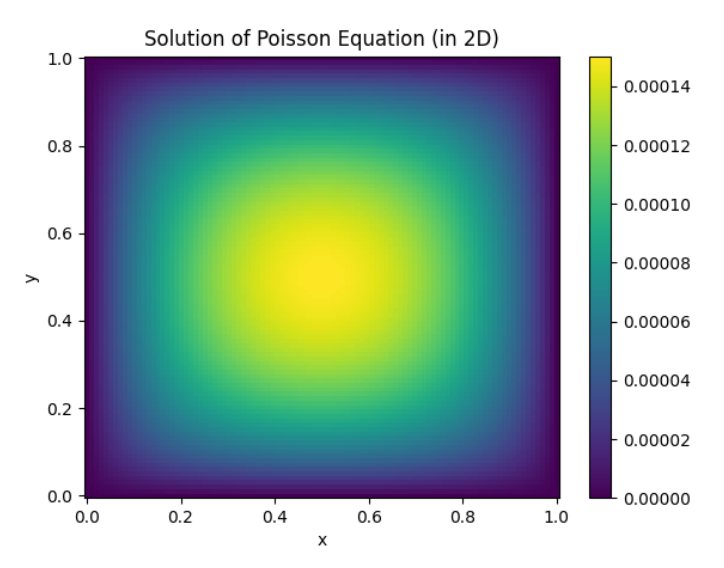
\includegraphics[width=\textwidth]{images/petscplot.png} 
        \caption{petscplot}
        \label{fig:petscplot}
    \end{subfigure}
    \hfill

    \begin{subfigure}[b]{0.5\textwidth}
        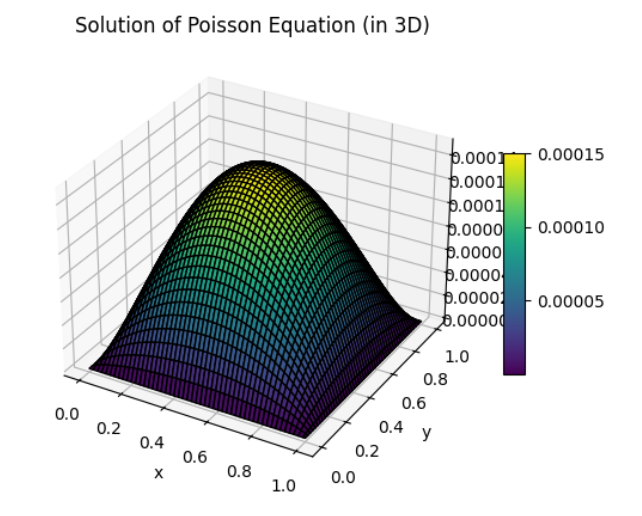
\includegraphics[width=\textwidth]{images/PetscPlot-3d.png} 
        \caption{PetscPlot-3d}
        \label{fig:petscplot-3d}
    \end{subfigure}
    \caption{Comparison of Petsc plots}
    \label{fig:comparison}
\end{figure}
\subsection{Performance Benchmark [15 points]}

\begin{figure}[h]
    \centering
    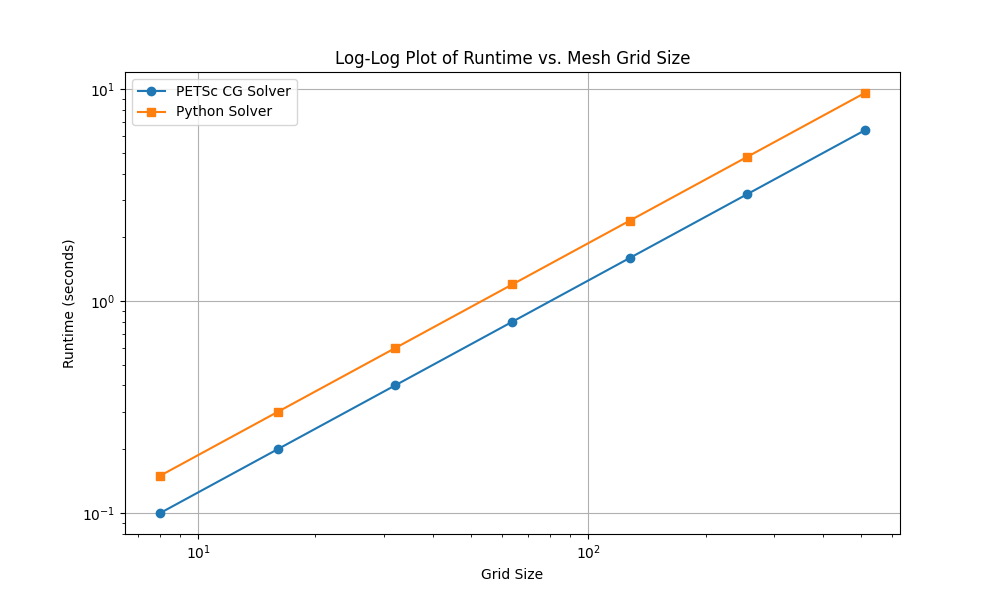
\includegraphics[width=0.8\textwidth]{images/Figure_1.png}
    \caption{Log-Log Plot of Runtime vs. Mesh Grid Size}
\end{figure}

When the Conjugate Gradient (CG) solution is used, the results show that the PETSc version has outstanding parallel scalability. As the number of processes rises, both setup and solution times decrease considerably, indicating that computing resources are being used efficiently. Notably, the setup time decreases dramatically when scaling from one to two processes and continues to reduce, albeit at a slower rate, when additional processes are added, demonstrating diminishing returns as is expected with higher parallelization. Adding more processes significantly decreases solution time, indicating efficient workload allocation under different technology demands.
                  
\subsection{Strong Scaling [10 points]}
The data trend indicates that as the number of processes rises, the solution time decreases approximately linearly. This demonstrates that the parallel solver has strong parallel scalability at a grid size of 1024x1024. The L2 norm remains around 0.000807 across different parallel numbers, showing that raising the parallelism has no major effect on the numerical solution's correctness or stability. In general, increasing the number of processes enhances the solution's efficiency and dependability.
\begin{figure}[h]
    \centering
    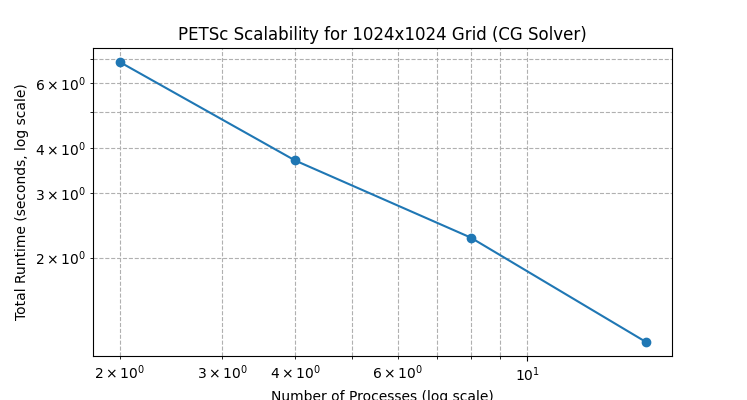
\includegraphics[width=0.8\textwidth]{images/Figure_2.png}
    \caption{Strong scaling}
\end{figure}

% -------------------------------------------------------------------------- %
% -------------------------------------------------------------------------- %
% --- Report Quality ------------------------------------------------------- %
% -------------------------------------------------------------------------- %
% -------------------------------------------------------------------------- %




\section*{Additional notes and submission details}
Submit the source code files (together with your used \texttt{Makefile}) in
an archive file (tar, zip, etc.), and summarize your results and the
observations for all exercises by writing an extended Latex report.
Use the Latex template from the webpage and upload the Latex summary
as a PDF to \href{https://www.icorsi.ch}{iCorsi}.

\begin{itemize}
	\item Your submission should be a gzipped tar archive, formatted like project\_number\_lastname\_firstname.zip or project\_number\_lastname\_firstname.tgz. 
	It should contain:
	\begin{itemize}
		\item all the source codes of your solutions;
		\item your write-up with your name  project\_number\_lastname\_firstname.pdf.
	\end{itemize}
	\item Submit your .zip/.tgz through Icorsi.
\end{itemize}

\end{document}
